\documentclass[10pt]{article}
\usepackage{tikz}
\usetikzlibrary{shapes.geometric}

\tikzstyle{monsterBody} = [regular polygon, regular polygon sides=3, fill, very thick, inner sep=1mm, below]
\tikzstyle{monsterHead} = [circle, fill, inner sep=1.5mm]

\newcommand{\hexagons}[3]{
        \foreach \i in {0,..., #2}
                \foreach \j in {0, 2,..., #3} {
			\path ({#1*\i},{#1*cos(30)*\j}) node[regular polygon, regular polygon sides=6, draw, thick, inner sep = {#1*10}, rotate = 90] {};
			\path ({#1*\i-#1/2},{#1*cos(30)*\j-#1*cos(30)}) node[regular polygon, regular polygon sides=6, draw, thick, inner sep = {#1*10}, rotate = 90] {};
			}
}

\newcommand{\monster}[4]{
	\ifodd#3
        	\path ({#1*#2-#1/2},{#1*cos(30)*#3}) node[monsterBody] [#4] {};
		\path ({#1*#2-#1/2},{#1*cos(30)*#3}) node[monsterHead] [#4] {};
	\else
        	\path ({#1*#2},{#1*cos(30)*#3}) node[monsterBody] [#4] {};
        	\path ({#1*#2},{#1*cos(30)*#3}) node[monsterHead] [#4] {};
	\fi
}

\newcommand{\arrow}[6]{
	\ifodd#3
		\def \i {({#1*#2-#1/2},{#1*cos(30)*#3})}
	\else
		\def \i {({#1*#2},{#1*cos(30)*#3})}
	\fi

	\ifodd#5
		\def \j {({#1*#4-#1/2},{#1*cos(30)*#5})}
	\else
		\def \j {({#1*#4},{#1*cos(30)*#5})}
	\fi

        \draw[->, ultra thick, #6] \i -- \j;
}

\newcommand{\background}[4]{
	\ifodd#3
		\path ({#1*#2-#1/2},{#1*cos(30)*#3}) node[regular polygon, regular polygon sides=6, draw, thick, inner sep = {#1*10}, rotate = 90, fill=#4] {};
	\else
		\path ({#1*#2},{#1*cos(30)*#3}) node[regular polygon, regular polygon sides=6, draw, thick, inner sep = {#1*10}, rotate = 90, fill=#4] {};
	\fi
}

\begin{document}

\begin{center}\Huge
	Détails du principe du jeu
\end{center}

\tableofcontents

\section{Legende}

\begin{table}[!ht]
	\begin{center}
		\begin{tabular}{| c | c | c |}
			\hline
			& rouge & bleu \\ \hline
			monstre & 
\begin{tikzpicture}\monster{2}{0}{0}{red}\end{tikzpicture} & 
\begin{tikzpicture}\monster{2}{0}{0}{blue}\end{tikzpicture} \\ \hline
			déplacement & 
\begin{tikzpicture}\arrow{2}{0}{0}{1}{0}{red}\end{tikzpicture} & 
\begin{tikzpicture}\arrow{2}{0}{0}{1}{0}{blue}\end{tikzpicture} \\ \hline
			attaque & 
\begin{tikzpicture}\background{1}{0}{0}{orange}\end{tikzpicture} & 
\begin{tikzpicture}\background{1}{0}{0}{cyan}\end{tikzpicture} \\ \hline
			
		\end{tabular}
	\end{center}
\end{table}

\newpage

\section{Gestion avec déplacement uniquement}

\subsection{Cas 1}

\begin{table}[!ht]
	\begin{center}
		\begin{tabular}{c c c}
			\multicolumn{3}{c}{
				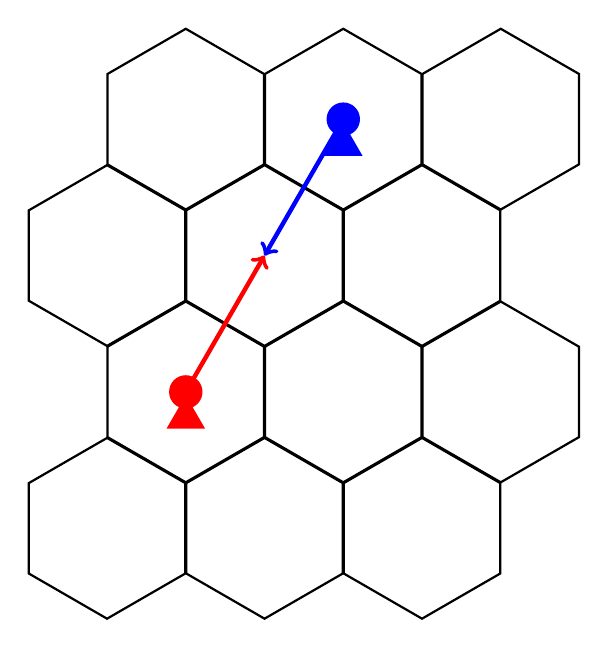
\begin{tikzpicture}
					\hexagons{2}{2}{2}
					\monster{2}{0}{0}{red}
					\monster{2}{1}{2}{blue}
					\arrow{2}{0}{0}{1}{1}{red}
					\arrow{2}{1}{2}{1}{1}{blue}
				\end{tikzpicture}} \\
			egalite & victoire de rouge & victoire de bleu \\
			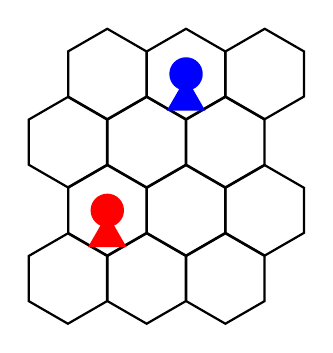
\begin{tikzpicture}\hexagons{1}{2}{2}\monster{1}{0}{0}{red}\monster{1}{1}{2}{blue}\end{tikzpicture} & 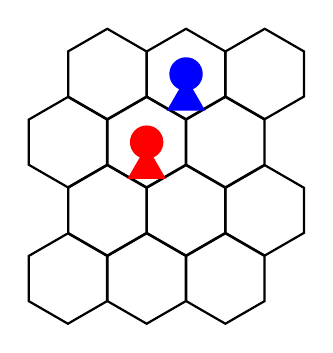
\begin{tikzpicture}\hexagons{1}{2}{2}\monster{1}{1}{1}{red}\monster{1}{1}{2}{blue}\end{tikzpicture} & 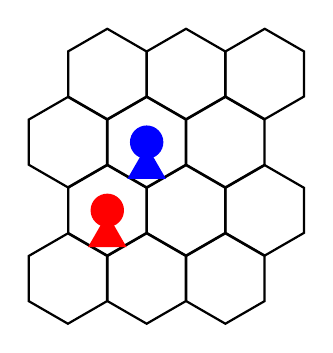
\begin{tikzpicture}\hexagons{1}{2}{2}\monster{1}{0}{0}{red}\monster{1}{1}{1}{blue}\end{tikzpicture} \\
			rouge et bleu blessés & bleu blessé & rouge blessé \\
			\multicolumn{3}{c}{tout autre attaque est annulé}
		\end{tabular}
	\end{center}
\end{table}

\newpage

\subsection{Cas 2}

\begin{table}[!ht]
	\begin{center}
		\begin{tabular}{c c c}
			\multicolumn{3}{c}{
				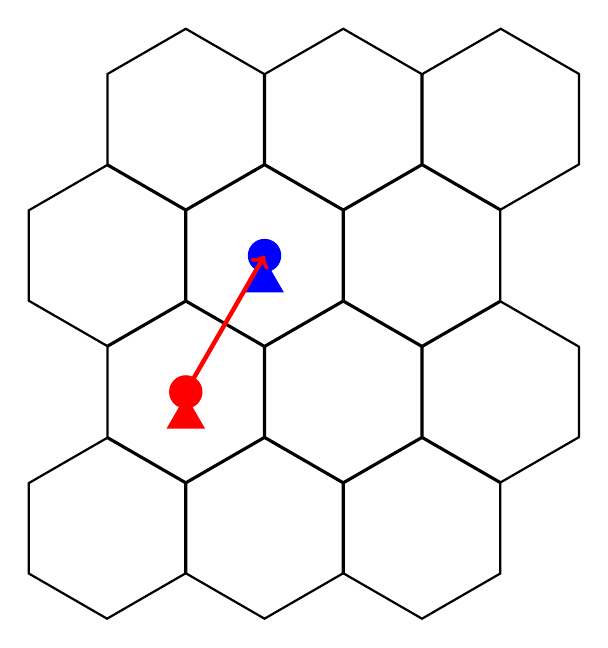
\begin{tikzpicture}
					\hexagons{2}{2}{2}
					\monster{2}{0}{0}{red}
					\monster{2}{1}{1}{blue}
					\arrow{2}{0}{0}{1}{1}{red}
				\end{tikzpicture}} \\
			egalite & victoire de rouge & victoire de bleu \\
			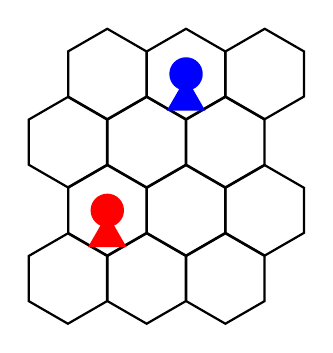
\begin{tikzpicture}\hexagons{1}{2}{2}\monster{1}{0}{0}{red}\monster{1}{1}{2}{blue}\end{tikzpicture} & 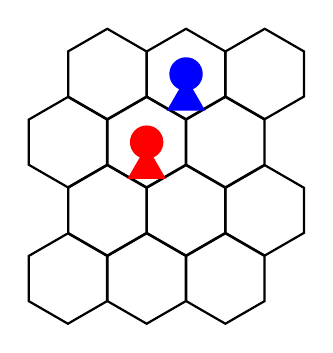
\begin{tikzpicture}\hexagons{1}{2}{2}\monster{1}{1}{1}{red}\monster{1}{1}{2}{blue}\end{tikzpicture} & 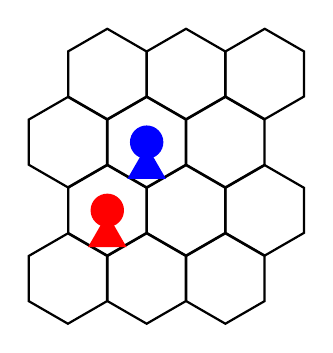
\begin{tikzpicture}\hexagons{1}{2}{2}\monster{1}{0}{0}{red}\monster{1}{1}{1}{blue}\end{tikzpicture} \\
			rouge et bleu blessés & bleu blessé & rouge blessé \\
			\multicolumn{3}{c}{tout autre attaque est annulé}
		\end{tabular}
	\end{center}
\end{table}

\newpage

\subsection{Cas 3}

\begin{table}[!ht]
	\begin{center}
		\begin{tabular}{c}
			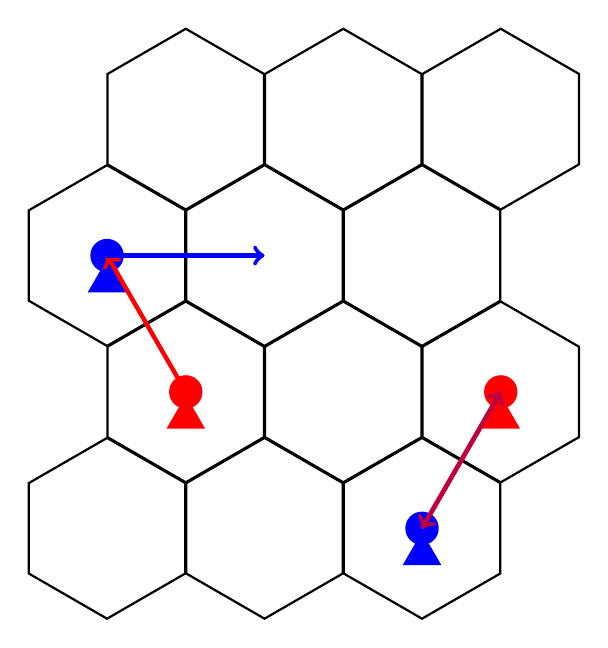
\begin{tikzpicture}
				\hexagons{2}{2}{2}
				\monster{2}{0}{0}{red}
				\monster{2}{0}{1}{blue}
				\monster{2}{2}{0}{red}
				\monster{2}{2}{-1}{blue}
				\arrow{2}{0}{0}{0}{1}{red}
				\arrow{2}{0}{1}{1}{1}{blue}
				\arrow{2}{2}{0}{2}{-1}{purple}
				\arrow{2}{2}{-1}{2}{0}{purple}
			\end{tikzpicture} \\
			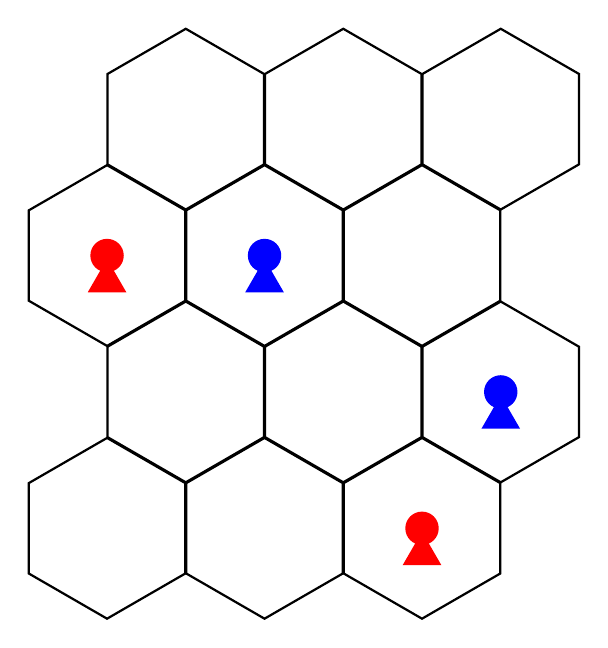
\begin{tikzpicture}
				\hexagons{2}{2}{2}
				\monster{2}{0}{1}{red}
				\monster{2}{1}{1}{blue}
				\monster{2}{2}{-1}{red}
				\monster{2}{2}{0}{blue}
			\end{tikzpicture} \\
			les attaques sont ensuite traités
		\end{tabular}
	\end{center}
\end{table}

\newpage

\subsection{Cas impossibles}

\begin{table}[!ht]
	\begin{center}
		\begin{tabular}{c}
			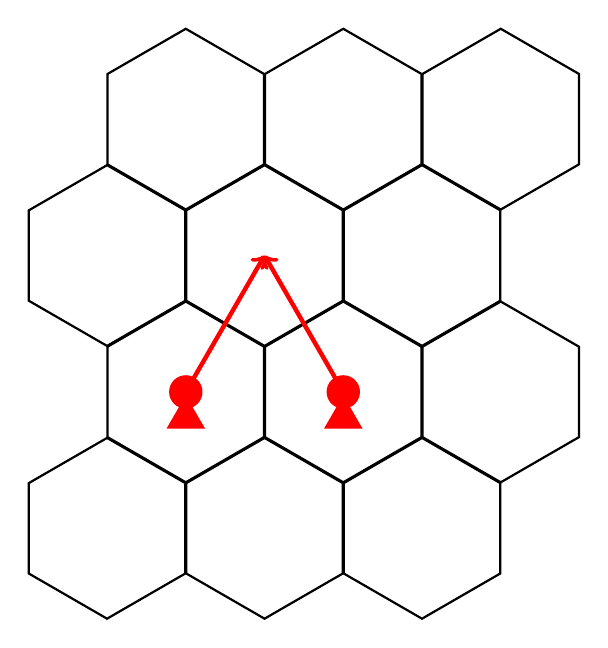
\begin{tikzpicture}
				\hexagons{2}{2}{2}
				\monster{2}{0}{0}{red}
				\monster{2}{1}{0}{red}
				\arrow{2}{0}{0}{1}{1}{red}
				\arrow{2}{1}{0}{1}{1}{red}
			\end{tikzpicture} \\
		\end{tabular}
	\end{center}
\end{table}

\newpage

\section{Gestion avec attaque uniquement}

\subsection{Cas 1}

\begin{table}[!ht]
	\begin{center}
		\begin{tabular}{c}
			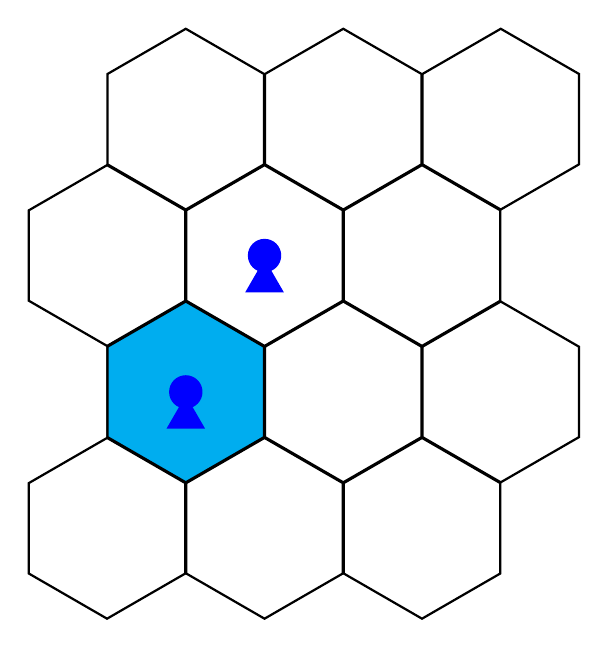
\begin{tikzpicture}
				\hexagons{2}{2}{2}
				\background{2}{0}{0}{cyan}
				\monster{2}{0}{0}{blue}
				\monster{2}{1}{1}{blue}
			\end{tikzpicture} \\
			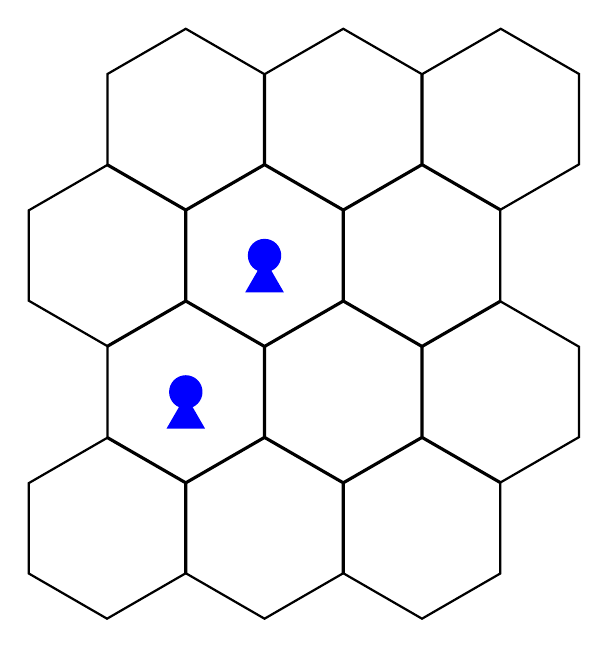
\begin{tikzpicture}
				\hexagons{2}{2}{2}
				\monster{2}{0}{0}{blue}
				\monster{2}{1}{1}{blue}
			\end{tikzpicture} \\
			si le bleu en bas est plus faible que celui du haut,\\ il prend un point de dégat sinon il ne se passe rien
		\end{tabular}
	\end{center}
\end{table}

\newpage

\subsection{Cas 2}

\begin{table}[!ht]
	\begin{center}
		\begin{tabular}{c c c}
			\multicolumn{3}{c}{
				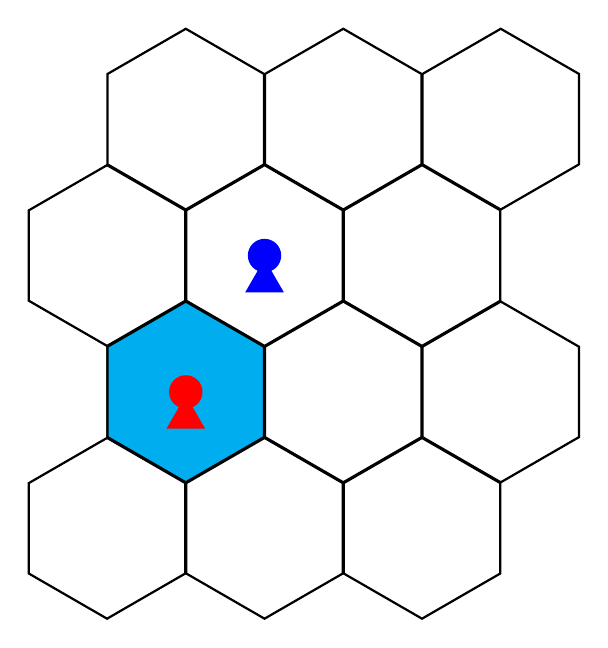
\begin{tikzpicture}
					\hexagons{2}{2}{2}
					\background{2}{0}{0}{cyan}
					\monster{2}{0}{0}{red}
					\monster{2}{1}{1}{blue}
				\end{tikzpicture}} \\
			egalite & victoire de rouge & victoire de bleu \\
			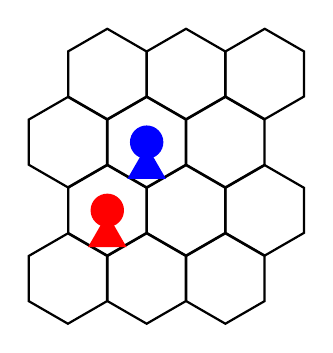
\begin{tikzpicture}\hexagons{1}{2}{2}\monster{1}{0}{0}{red}\monster{1}{1}{1}{blue}\end{tikzpicture} & 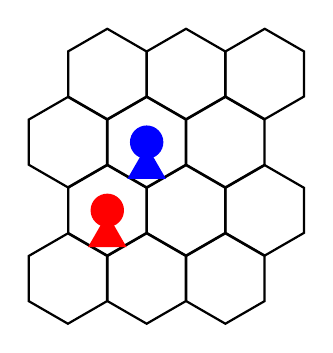
\begin{tikzpicture}\hexagons{1}{2}{2}\monster{1}{0}{0}{red}\monster{1}{1}{1}{blue}\end{tikzpicture} & 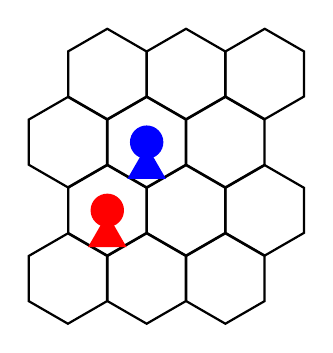
\begin{tikzpicture}\hexagons{1}{2}{2}\monster{1}{0}{0}{red}\monster{1}{1}{1}{blue}\end{tikzpicture} \\
			rouge blessés & rien ne se passe & rouge blessé \\
		\end{tabular}
	\end{center}
\end{table}

\newpage

\subsection{Cas 3}

\begin{table}[!ht]
	\begin{center}
		\begin{tabular}{c c c}
			\multicolumn{3}{c}{
				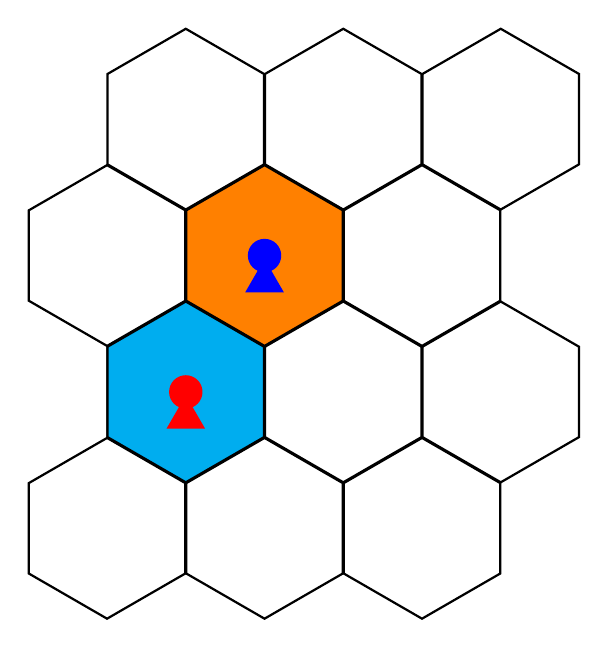
\begin{tikzpicture}
					\hexagons{2}{2}{2}
					\background{2}{1}{1}{orange}
					\background{2}{0}{0}{cyan}
					\monster{2}{0}{0}{red}
					\monster{2}{1}{1}{blue}
				\end{tikzpicture}} \\
			egalite & victoire de rouge & victoire de bleu \\
			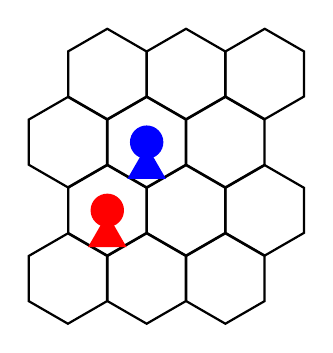
\begin{tikzpicture}\hexagons{1}{2}{2}\monster{1}{0}{0}{red}\monster{1}{1}{1}{blue}\end{tikzpicture} & 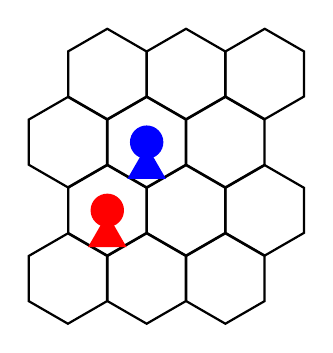
\begin{tikzpicture}\hexagons{1}{2}{2}\monster{1}{0}{0}{red}\monster{1}{1}{1}{blue}\end{tikzpicture} & 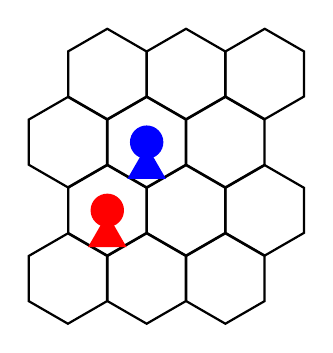
\begin{tikzpicture}\hexagons{1}{2}{2}\monster{1}{0}{0}{red}\monster{1}{1}{1}{blue}\end{tikzpicture} \\
			rouge et bleu blessés & bleu blessé & rouge blessé \\
		\end{tabular}
	\end{center}
\end{table}

\newpage

\subsection{Cas 4}

\begin{table}[!ht]
	\begin{center}
		\begin{tabular}{c c c}
			\multicolumn{3}{c}{
				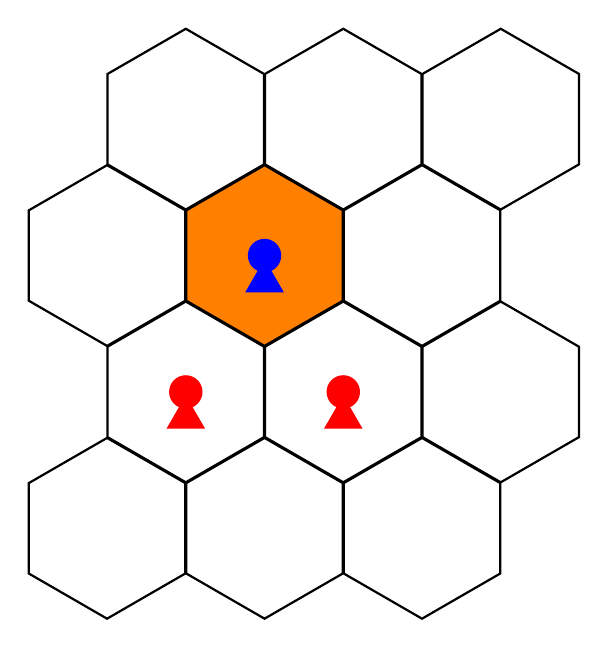
\begin{tikzpicture}
					\hexagons{2}{2}{2}
					\background{2}{1}{1}{orange}
					\monster{2}{0}{0}{red}
					\monster{2}{1}{0}{red}
					\monster{2}{1}{1}{blue}
				\end{tikzpicture}} \\
			\multicolumn{3}{c}{les deux rouges attaquent le bleu}\\
			\multicolumn{3}{c}{on compare l'attaque du bleu avec la somme de celle de chacun des rouges}\\
			egalite & victoire de rouge & victoire de bleu \\
			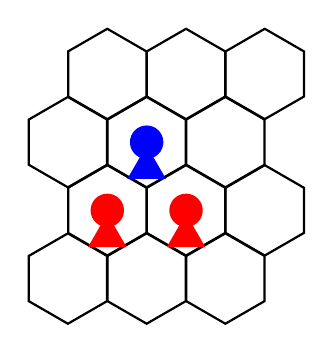
\begin{tikzpicture}\hexagons{1}{2}{2}\monster{1}{0}{0}{red}\monster{1}{1}{0}{red}\monster{1}{1}{1}{blue}\end{tikzpicture} & 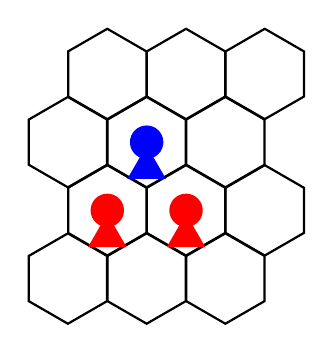
\begin{tikzpicture}\hexagons{1}{2}{2}\monster{1}{0}{0}{red}\monster{1}{1}{0}{red}\monster{1}{1}{1}{blue}\end{tikzpicture} & 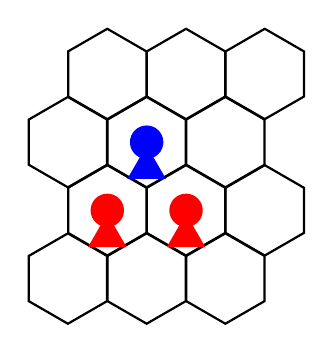
\begin{tikzpicture}\hexagons{1}{2}{2}\monster{1}{0}{0}{red}\monster{1}{1}{0}{red}\monster{1}{1}{1}{blue}\end{tikzpicture} \\
			bleu blessé & bleu blessé & rien ne se passe \\
		\end{tabular}
	\end{center}
\end{table}

\newpage

\section{Gestion mixte déplacement et attaque}

\subsection{Cas 1}

\begin{table}[!ht]
	\begin{center}
		\begin{tabular}{c c c}
			\multicolumn{3}{c}{
				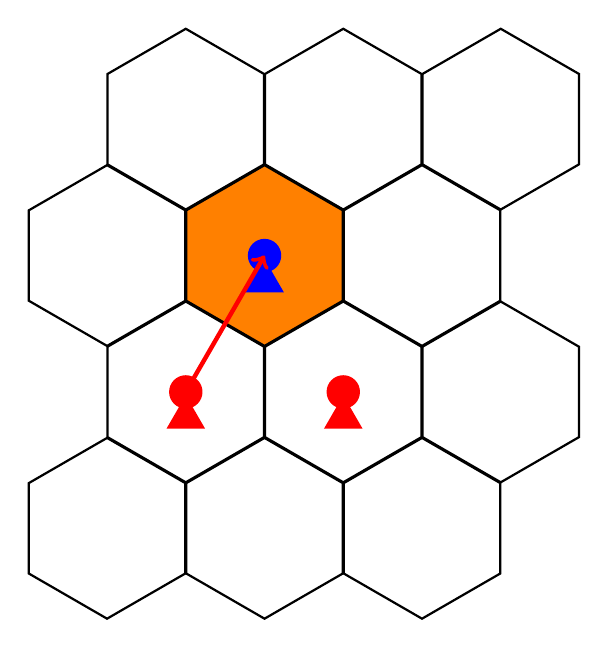
\begin{tikzpicture}
					\hexagons{2}{2}{2}
					\background{2}{1}{1}{orange}
					\monster{2}{0}{0}{red}
					\monster{2}{1}{0}{red}
					\monster{2}{1}{1}{blue}
					\arrow{2}{0}{0}{1}{1}{red}
				\end{tikzpicture}} \\
			\multicolumn{3}{c}{les deux rouges attaquent le bleu}\\
			\multicolumn{3}{c}{on compare l'attaque du bleu avec la somme de celle de chacun des rouges}\\
			egalite & victoire de rouge & victoire de bleu \\
			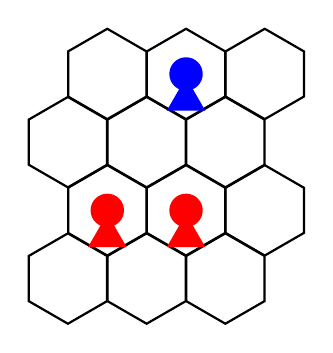
\begin{tikzpicture}\hexagons{1}{2}{2}\monster{1}{0}{0}{red}\monster{1}{1}{0}{red}\monster{1}{1}{2}{blue}\end{tikzpicture} & 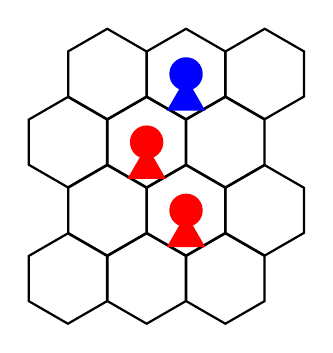
\begin{tikzpicture}\hexagons{1}{2}{2}\monster{1}{1}{1}{red}\monster{1}{1}{0}{red}\monster{1}{1}{2}{blue}\end{tikzpicture} & 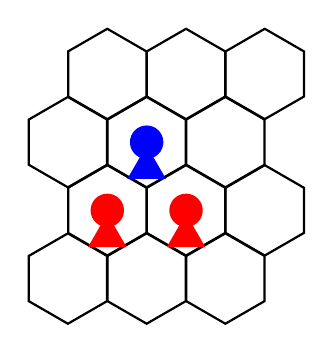
\begin{tikzpicture}\hexagons{1}{2}{2}\monster{1}{0}{0}{red}\monster{1}{1}{0}{red}\monster{1}{1}{1}{blue}\end{tikzpicture} \\
			le rouge de gauche & bleu blessé & le rouge de gauche \\
			et bleu blessés && blessé 
		\end{tabular}
	\end{center}
\end{table}

\newpage

\section{Pouvoir spéciaux}

\subsection{Si les mouvements sont annulés}

\begin{table}[!ht]
	\begin{center}
		\begin{tabular}{c}
			Situation de départ \\
			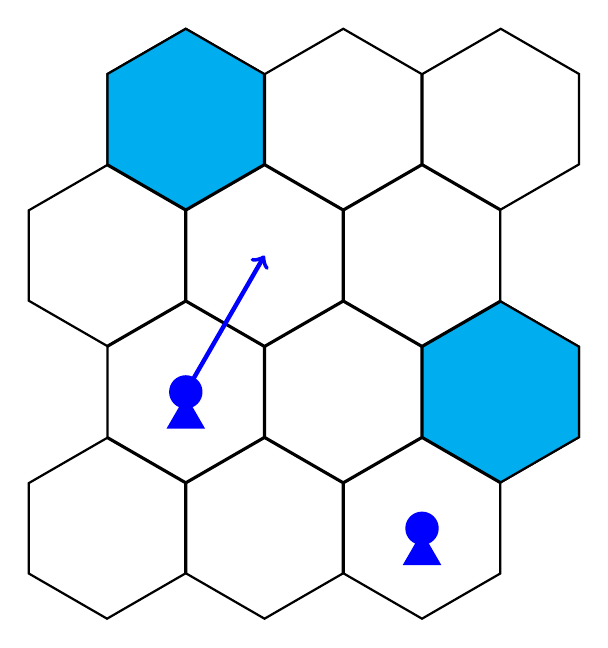
\begin{tikzpicture}
				\hexagons{2}{2}{2}
				\background{2}{0}{2}{cyan}
				\background{2}{2}{0}{cyan}
				\monster{2}{0}{0}{blue}
				\monster{2}{2}{-1}{blue}
				\arrow{2}{0}{0}{1}{1}{blue}
			\end{tikzpicture} \\
			Situation réellement traité \\
			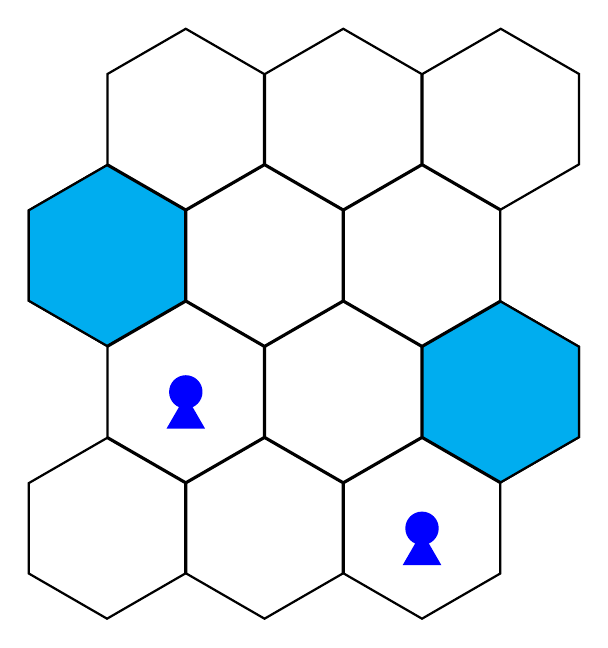
\begin{tikzpicture}
				\hexagons{2}{2}{2}
				\background{2}{0}{1}{cyan}
				\background{2}{2}{0}{cyan}
				\monster{2}{0}{0}{blue}
				\monster{2}{2}{-1}{blue}
			\end{tikzpicture} 
		\end{tabular}
	\end{center}
\end{table}

\newpage

\section{Type d'attaque}

\begin{table}[!ht]
	\begin{center}
		\begin{tabular}{c c}
			attaque 1 & 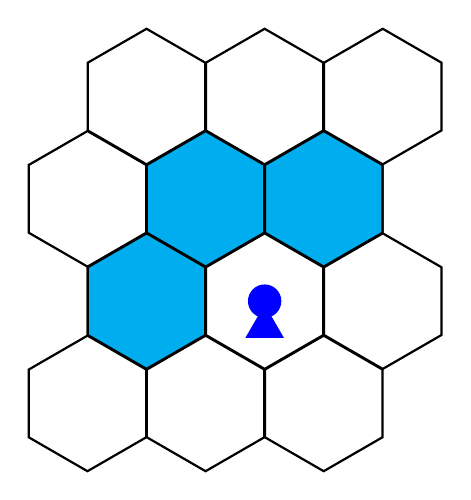
\begin{tikzpicture}
				\hexagons{1.5}{2}{2}
				\background{1.5}{0}{0}{cyan}
				\background{1.5}{1}{1}{cyan}
				\background{1.5}{2}{1}{cyan}
				\monster{1.5}{1}{0}{blue}
			\end{tikzpicture} \\
			attaque 2 & 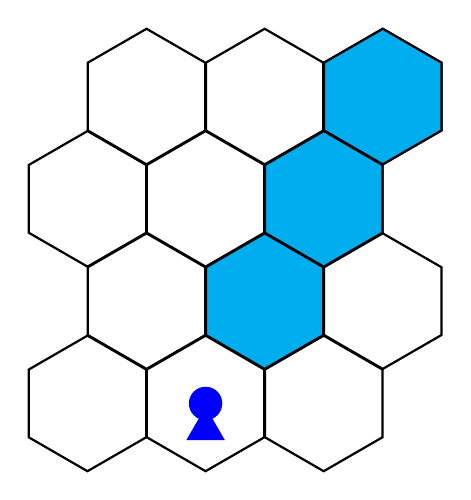
\begin{tikzpicture}
				\hexagons{1.5}{2}{2}
				\background{1.5}{1}{0}{cyan}
				\background{1.5}{2}{1}{cyan}
				\background{1.5}{2}{2}{cyan}
				\monster{1.5}{1}{-1}{blue}
			\end{tikzpicture} \\
			attaque 3 & 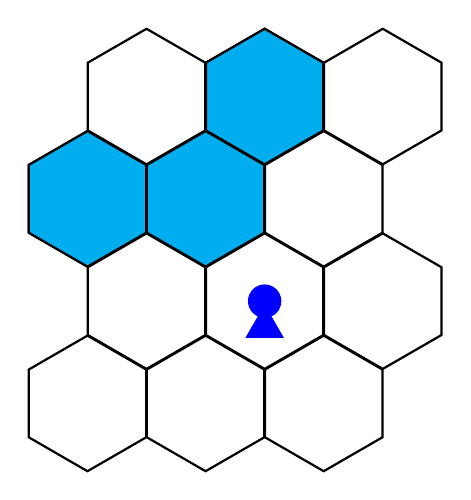
\begin{tikzpicture}
				\hexagons{1.5}{2}{2}
				\background{1.5}{0}{1}{cyan}
				\background{1.5}{1}{1}{cyan}
				\background{1.5}{1}{2}{cyan}
				\monster{1.5}{1}{0}{blue}
			\end{tikzpicture}
		\end{tabular}
	\end{center}
\end{table}

\section{Condition de victoire}

\subsection{proposition 1}

Prendre le contrôle des différentes cases clefs

\subsection{proposition 2}

Détruire la base adverse

\subsection{proposition 3}

Emmener un objet près la base adverse

\subsection{proposition 4}



\end{document}
